\section{Цель работы}
Реализовать и исследовать метод Монте-Карло для численного вычисления заданного двойного интеграла, сравнить полученные приближенные значения с точным значением интеграла и оценить эффективность метода при различных значениях количества случайных точек.
\section{Содержание работы}
\begin{enumerate}
	\item Изучить метод Монте-Карло для кратных интегралов;
	\item Записать заданный двойной интеграл в приведенном виде;
	\item Составить программу, реализующую вычисление интеграла при \(N=20,50,100\). Вывести на печать полученные значения интеграла. Для случая \(N=20\) вывести на печать также координаты случайных точек, значения подынтегральной функции в этих точках и информацию о принадлежности точек области интегрирования;
	\item Сравнить полученные с помощью программы приближенные значения интеграла с его точным значением, найденным непосредственным вычислением.
\end{enumerate}

\section{Выполнение работы}
\subsection{Задание}
Найти кратный интеграл
\begin{align}
	\iint\limits_D(2x+y)dxdy,
\end{align}
где \(D\) --- область, ограниченная гиперболой \(xy=8\) и прямыми \(y-2x = 0\) и \(x=6\).
\begin{figure}[h]
	\centering
	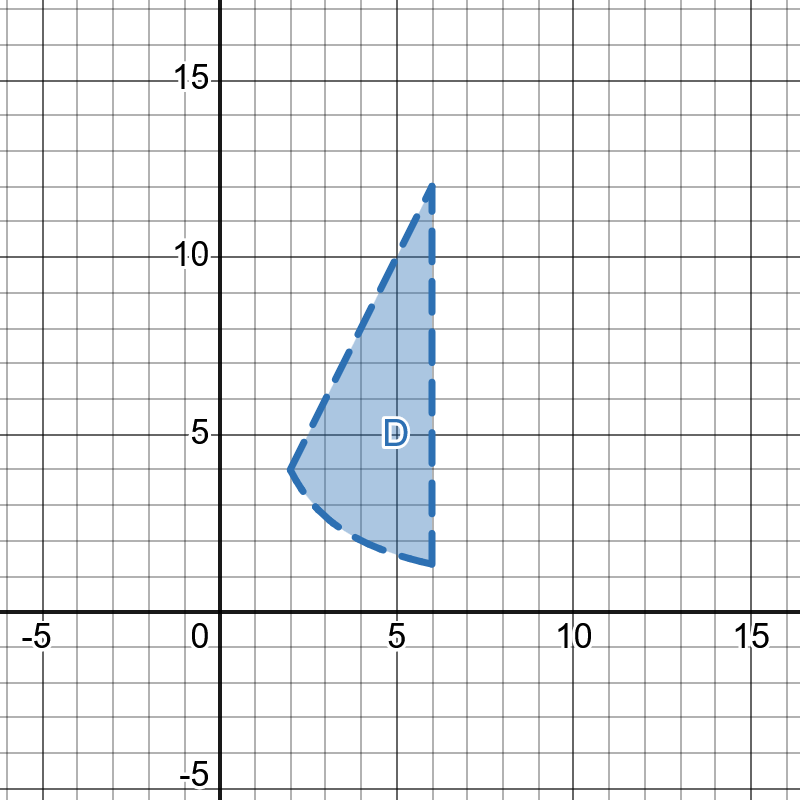
\includegraphics[height=6cm]{DD1}
	\caption{Область \(D\)}
\end{figure}
\subsection{Прямое вычисление интеграла}

\begin{multline}
	\iint\limits_D(2x+y)dxdy = \int_2^6\int_{8/x}^{2x} (2x+y) dy dx = \int_2^6 \roundbrac{2xy\Bigr|_{8/x}^{2x} + \frac{y^2}{2}\Bigr|_{8/x}^{2x} }dx = \\
	= \int_2^6 \roundbrac{4x^2 - 16 + \frac{4x^2}{2} - \frac{64}{2x^2}} = \int_2^6\roundbrac{
		2x^2-16-\frac{32}{x^2}}dx = 2x^3\Bigr|_2^6 - 16x\Bigr|_2^6 + \frac{32}{x}\Bigr|_2^6 =\\
	= \frac{1024}{3} \approx 341.(3)
\end{multline}

\subsection{Приведение интеграла}
Метод Монте-Карло основан на аппроксимации интеграла с помощью среднего значения функции, вычисленного в случайных точках. Для удобства генерации таких точек и обеспечения их равномерного распределения, область интегрирования отображается на единичный куб \([0,1]^n\). Это преобразование позволяет использовать стандартные генераторы случайных чисел, равномерно распределенных в диапазоне \([0,1]\).

Так рассмотрим область \([a, A] \times [b, B] \supset D\), мы хотим задать отображение, причем следующее:
\begin{align}
	\varphi \colon R^2 \to R^2 \\
	\varphi \colon [0, 1]^2 \mapsto [a, A] \times [b, B]
\end{align}
Задать такое преобразование можно как аффинное. А раз преобразование аффинное, то оно является и диффеоморфизмом. А значит мы можем использовать формулу замены переменных.
\begin{align}
	\int\limits_{D=\varphi(D')}f(x)dx = \int\limits_{D'}f(\varphi(t))|\varphi'(t)|dt
\end{align}
При том \(|\varphi'(t)| = |J_t\varphi|\) --- якобиан преобразования \(\varphi\).

Более конкретно, задаем замену:
\begin{align}
	\begin{cases}
		x = a + (A - a) \xi \\
		y = b + (B - b) \eta
	\end{cases}
\end{align}
Тогда якобиан:
\begin{align}
	|\varphi'| = \begin{vmatrix}
		             x'_\xi & x'_\eta \\
		             y'_\xi & y'_\eta
	             \end{vmatrix} = \begin{vmatrix}
		                             A - a & 0     \\
		                             0     & B - b
	                             \end{vmatrix} = (A - a) (B - b)
\end{align}
Интеграл принимает вид:
\begin{align}\label{eq:ab-iint}
	I = (A - a)(B - b)\iint\limits_{D'}f(\varphi(t))dt
\end{align}
А для заданного примера:
\begin{align}
	\begin{cases}
		x = 2 + 4 \xi \\
		y = \frac{4}{3} + \frac{32}{3} \eta
	\end{cases}
\end{align}
\begin{align}
	I = \frac{128}{9}\iint\limits_{D'}(16 + 24\xi + 32\eta)d\xi d\eta
\end{align}
Где
\begin{align}
	D'\colon \begin{cases}
		         \xi < 1      \\
		         4\eta-3\xi<1 \\
		         (2+4\xi)(4+32\eta)>24
	         \end{cases}
\end{align}

\begin{figure}[h]
	\begin{subfigure}{.5\textwidth}
		\centering
		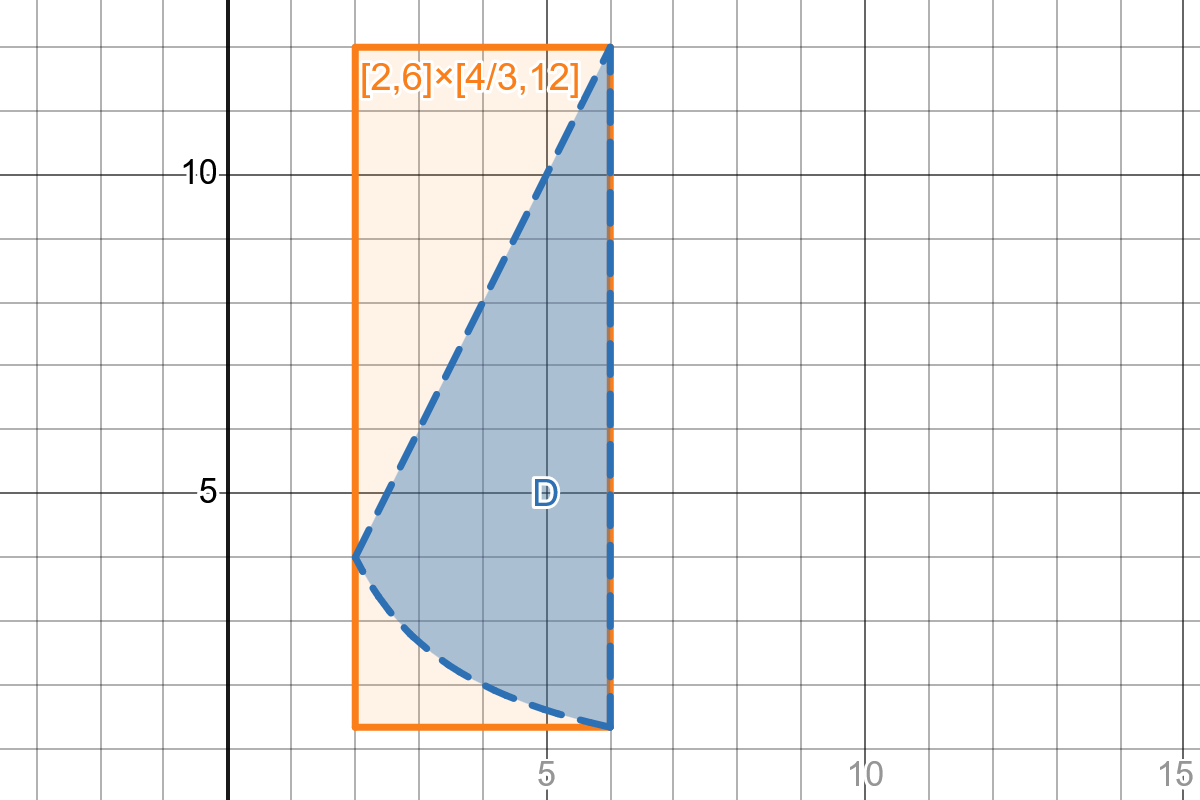
\includegraphics[width=.8\linewidth]{D-D1.png}
		\caption{Область \(D\)}
	\end{subfigure}
	\begin{subfigure}{.5\textwidth}
		\centering
		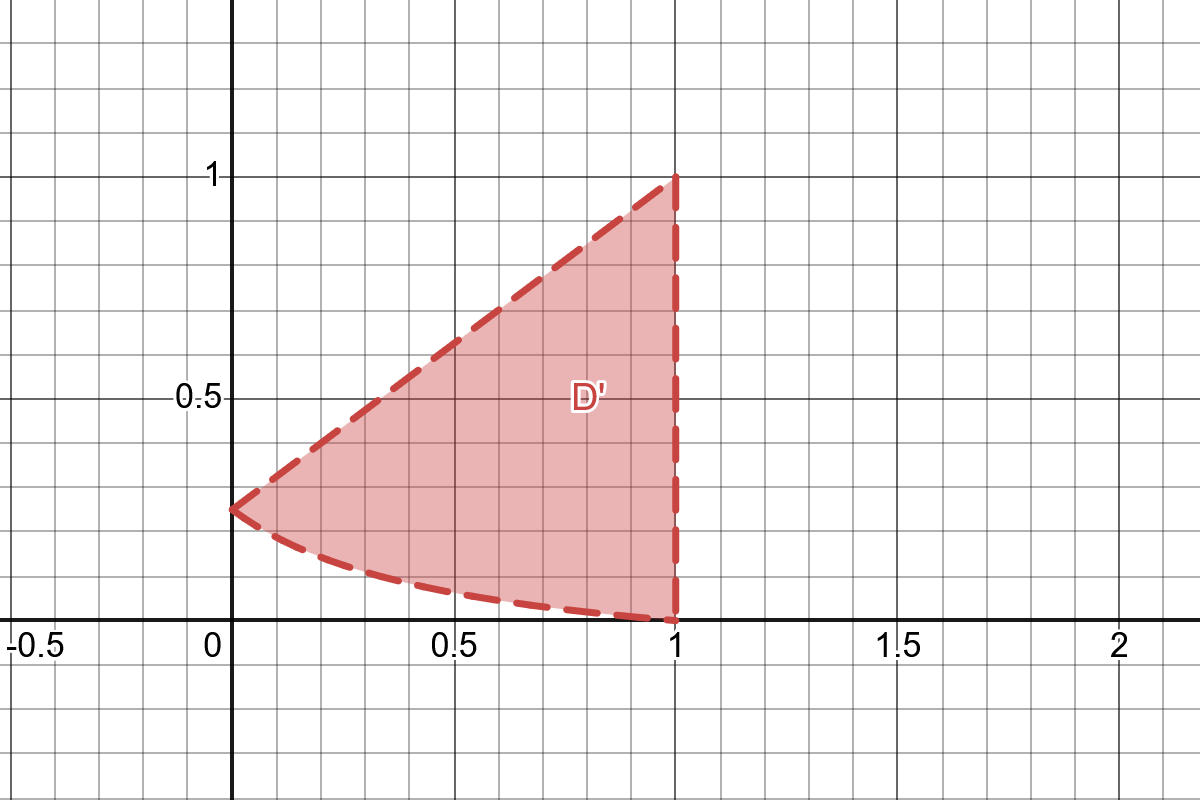
\includegraphics[width=.8\linewidth]{D1.png}
		\caption{Область \(D'\)}
	\end{subfigure}
\end{figure}

\subsection{Введение вероятностной модели}\label{method-1}
При условии, что \(f\circ\varphi\) неотрицательно на области \(D'\), данное тождество истинно:
\begin{align}
	f(\varphi(t)) = \int_0^{f(\varphi(t))}dr.
\end{align}
Допустив
\begin{align}
	0 \leq f(\varphi(t)) \leq R \Longrightarrow 0 \leq \frac{f(\varphi(t))}{R} \leq 1, \forall t \in D',
\end{align}
можно сделать замену
\begin{align}
	u = r R \Longrightarrow du = R dr \\
	r_a = 0, r_b = f(\varphi(t))/R.
\end{align}
Интеграл \cref{eq:ab-iint} принимает вид:
\begin{align}
	I = (A - a)(B - b)R\iint\limits_{D'}\int_0^{f(\varphi(t))/R}drdt = (A - a)(B - b)R \iiint\limits_{D''}d\xi,
\end{align}
где \(D'' \subset [0,1]^3\) находится над гиперплоскостью \(z = 0\) и под гиперповерхностью \(z =f(\varphi(t))\)

Для вероятностного пространства \((\Omega, F, P)\):
\begin{enumerate}
	\item \(\Omega = [0,1]^3 \subset \mathbb{R}^3\) --- множество элементарных событий;
	\item \(F\) --- \(\sigma\) алгебра подмножеств множества \(\Omega\), для которых введена мера \(\mu\);
	\item Вероятность \(P\) задается следующим образом:
	      \begin{align*}
		      P(X) = \frac{\mu(X)}{\mu(\Omega)} = \frac{\mu(X)}{1} = \mu(X)
	      \end{align*}
\end{enumerate}
Задача оценки интеграла как меры сводится к оценке вероятности попадания случайно выбранной точки из \(\Omega\) в область \(D''\).

Согласно теореме Бернулли, частота \(p^*\) появления события \(A\) сходится по вероятности к вероятности \(p\):
\begin{align}
	\lim_{n\to\infty}P\{|p^* - p| < \varepsilon \} = 1
\end{align}

Пусть \(X_i\) --- индикаторная случайная величина \(I_{D''}(X_i)\). Тогда:
\begin{align}
	P(I_{D''}(X_i)=1) = \mu(D'') = I_0 \\
	M[X_i] = 0(1 - I_0) + 1 I_0 = I_0  \\
	D[X_i] = (0 - I_0)^2 (1 - I_0) + (1 - I_0)^2 I_0 = I_0(1-I_0) < \frac{1}{4}
\end{align}
Задав случайную величину \(S_n\):
\begin{align}
	p^* = \frac{1}{n}\sum_{i=0}^n P(I_{D''}(X_i) = 1) = S_n,
\end{align}
выходит:
\begin{align}
	M[S_n] = \frac{1}{n}M[\sum_{i=0}^n P(I_{D''}(X_i) = 1)] = \frac{1}{n}\sum_{i=0}^n M[P(I_{D''}(X_i) = 1)] = \frac{1}{n}\sum_{i=0}^n I_0 = \frac{n}{n}I_0 = I_0 \\
	D[S_n] = \frac{1}{n^2}D[\sum_{i=0}^n P(I_{D''}(X_i) = 1)] =  \frac{1}{n^2}\sum_{i=0}^n I_0(1-I_0) = \frac{(1 - I_0)I_0}{n} < \frac{1}{4n}
\end{align}
И неравенство Чебышева
\begin{align}
	P\{|X-m_x|<\varepsilon\} \geq 1 - \frac{D_x}{\varepsilon^2}
\end{align}
принимает вид:
\begin{align}
	P\{|p^* - p|<\varepsilon\} \geq 1 - \frac{I_0(1-I_0)}{\varepsilon^2 n} \geq 1 - \frac{1}{4 \varepsilon^2 n} \\
	\label{eq:garant}
	P\{|p^* - p|<\varepsilon\} = 1 - \delta
\end{align}
Приняв для данной оценки \(\varepsilon\) гарантийную вероятность \cref{eq:garant}, выводится, что условие имеет место быть при
\begin{align}
	\frac{1}{4 \varepsilon^2 n} = \delta \Longrightarrow \varepsilon = \frac{1}{2\sqrt{\delta n}}.
\end{align}
Итак, поведение величины \(\varepsilon\) описывается
\begin{align}\label{eq:o-desc}
	\varepsilon = O\left(\frac{1}{\sqrt{n}}\right).
\end{align}
И необходимое число испытаний тогда:
\begin{align}
	n = \frac{1}{4 \varepsilon^2 \delta}
\end{align}

\subsection{Исключение одной случайной величины}\label{method-2}
Если взять пространство \((\Omega, F, P)\) с
\begin{enumerate}
	\item \(\Omega = [0,1]^2 \subset R^2\);
	\item \(F\) --- \(\sigma\) алгебра подмножеств множества \(\Omega\), для которых введена мера \(\mu\);
	\item Вероятность \(P\) задается следующим образом:
	      \begin{align*}
		      P(X) = \frac{\mu(X)}{\mu(\Omega)} = \frac{\mu(X)}{1} = \mu(X)
	      \end{align*}
\end{enumerate}

и рассмотреть случайную велчину вида
\begin{align}
	Y = I_{D'}(X)f(X),
\end{align}
то получается:
\begin{align}
	M[Y] = \iint_{[0,1]^2} p(X) I(X) f(X) dX.
\end{align}

Из определения индикатора:
\begin{align}
	M[Y] = \iint_{D'} p(X)f(X) dX,
\end{align}
учитывая равномерное распределение
\begin{align}
	p(x) = \frac{1}{A} = 1,
\end{align}
выходит
\begin{align}
	M[Y] = \iint_{D'} f(X) dX = I_0.
\end{align}
Дисперсия вычисляется как
\begin{align}
	D[Y] = \mu_2[Y] = \alpha_2[Y] - (\alpha_1[Y])^2 = M[Y^2] - (M[Y])^2 \\
	M[Y^2] = \iint_{[0, 1]^2} p(X)(I_{D'}(X)f(X))^2 dX = \iint_{D'}f^2(X) dX
\end{align}

Случайная величина, заданная как сумма данных независимых случайных величин
\begin{align}
	S = \frac{1}{n}\sum_{k=0}^n Y
\end{align}
имеет характеристики:
\begin{align}
	M[S] = \frac{n}{n}I_0 = I_0 \\
	D[S] = \frac{n}{n^2} D[Y] = \frac{1}{n} D[y]
\end{align}

Подставляя в неравеснтво Чебышева:
\begin{align}
	P\{|S - I_0|<\varepsilon\} \geq 1 - \frac{\iint_{D'}f^2(X)dX - I_0^2}{\varepsilon^2 n}. \\
\end{align}

Как итог
\begin{align}
	\lim_{n\to\infty}P\{|S - I_0|<\varepsilon\} = 1.
\end{align}
Асимптотически величина \(\varepsilon\) описывается так же, как и в формуле (\ref{eq:o-desc}).

\section{Вычисления}
\subsection{Пример вычисления}
Для \(N = 20\) рассматривается выборка точек с ее содержимым:

\begin{align*}
	\begin{array}{ll}
		(0.56763554 0.0789485) \to 457.23883   & (0.74630606 0.6721467) \to 788.1961   \\
		(0.43813038 0.57967687) \not\in D      & (0.34509814 0.5507567) \not\in D      \\
		(0.14233947 0.4783113) \not\in D       & (0.032078028 0.31770563) \not\in D    \\
		(0.8451768 0.15828753) \to 588.081     & (0.37217999 0.48739147) \to 576.4103  \\
		(0.48926282 0.085366964) \to 433.40872 & (0.2324897 0.54943454) \not\in D      \\
		(0.8560116 0.7436471) \to 858.1829     & (0.4741887 0.977206) \not\in D        \\
		(0.6843517 0.65986276) \to 761.45844   & (0.79020524 0.92588997) \not\in D     \\
		(0.17501795 0.9010966) \not\in D       & (0.59115267 0.17000258) \to 506.70572 \\
		(0.51510084 0.84061956) \not\in D      & (0.8522557 0.82952595) \to 895.9853   \\
		(0.8507035 0.46353948) \to 728.8909    & (0.56606627 0.77454865) \not\in D     \\
	\end{array}
\end{align*}
\begin{align*}
	I = \frac{1}{20}\sum_{k=0}^{10}=\frac{1}{20}( & 457.23883+588.081+433.40872+                     \\
	+                                             & 858.1829+761.45844+728.8909+                     \\
	+                                             & 788.1961+576.4103+506.70572+895.9853) = 329.7279
\end{align*}

\subsection{Отклонения}
Взяв для каждой конфигурации, для каждого \(N\), выборки в количестве \(K\) с размером каждой выборки \(K_i = K_0\) производятся вычисления:
\begin{enumerate}
	\item Вычисляется нормальное отклонение для каждой выборки
	      \begin{align}
		      \sigma_i = \sqrt{\frac{1}{K_i}\sum_{j=0}^{K_i} (x_k - \overline{x})^2}, i=\overline{0,K}
	      \end{align}
	\item Находится среднее значение среди полученных нормальных отклонений:
	      \begin{align}
		      m_\sigma = \frac{1}{K}\sum_{i=0}^K \sigma_i
	      \end{align}
	\item А так же нормальное отклонение среди полученных:
	      \begin{align}
		      \sigma_\sigma = \sqrt{\frac{1}{K}\sum_{i=0}^K(\sigma - \sigma_i)^2}
	      \end{align}
\end{enumerate}
Для вычислений взяты значения \(K=30\), \(K_0=100\).
\begin{table}[h!]
	\centering
	\begin{tabular}{|l|c|c|c|c|c|}
		\hline
		$N$     & $m_{\sigma1}$ & $\sigma_{\sigma1}$ & $m_{\sigma2}$  & $\sigma_{\sigma2}$ \\
		\hline
		$  20 $ & $  74.08163 $ & $ 4.6014333 $      & $ 109.821976 $ & $  7.773065 $      \\
		$  50 $ & $  46.76052 $ & $ 3.2611177 $      & $    68.9947 $ & $ 4.8407636 $      \\
		$ 100 $ & $ 32.825172 $ & $   2.68074 $      & $  47.794693 $ & $ 3.8238974 $      \\
		$ 200 $ & $ 22.975714 $ & $  1.596667 $      & $  34.144722 $ & $ 3.1301556 $      \\
		$ 300 $ & $ 19.188334 $ & $ 1.2513237 $      & $  27.316946 $ & $ 2.0922694 $      \\
		$ 400 $ & $ 17.110592 $ & $ 1.4182564 $      & $  24.498312 $ & $ 1.6277343 $      \\
		$ 500 $ & $ 14.788441 $ & $ 0.9899412 $      & $  21.324444 $ & $ 1.7795098 $      \\
		\hline
	\end{tabular}
\end{table}
\begin{figure}[h!]
	\hspace{-2em}
	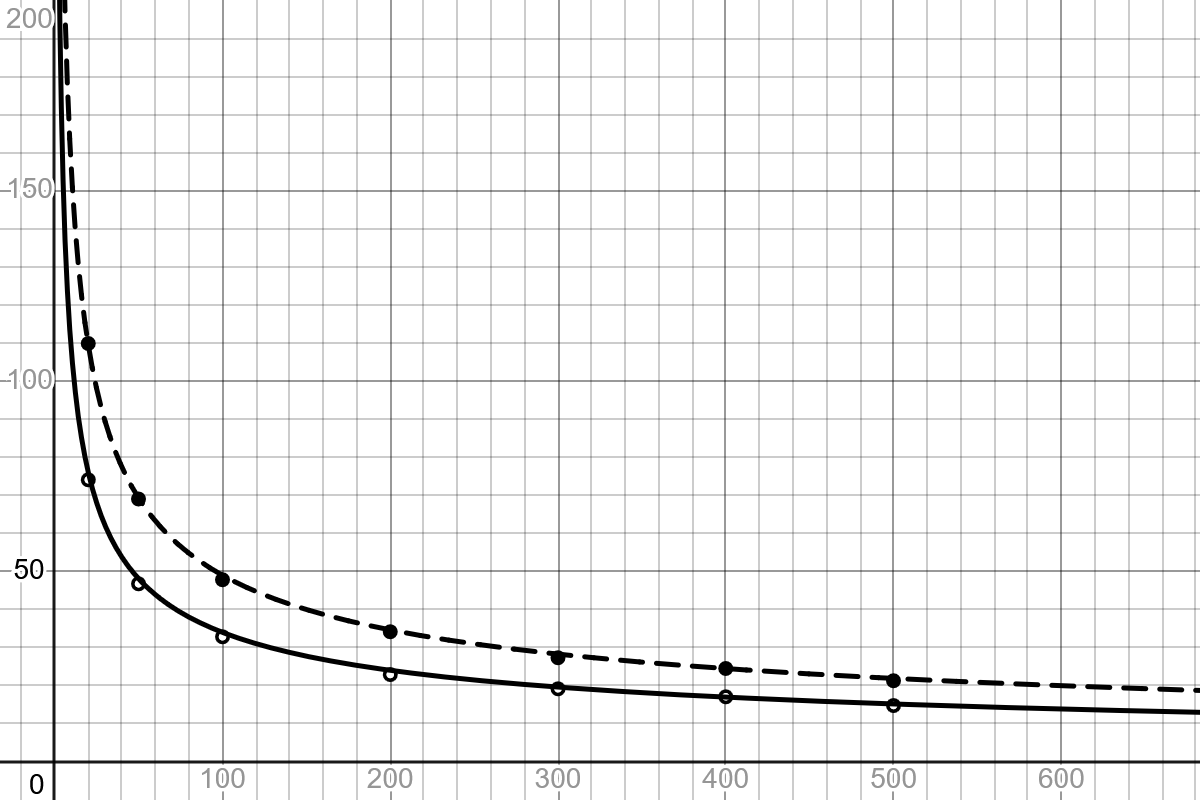
\includegraphics[width=\linewidth]{graphics/desmos-graph.png}
\end{figure}

% +-----+-----------+-----------+
% | N   | mₓ        | dₓ        |
% +-----+-----------+-----------+
% |  20 |  74.08163 | 4.6014333 |
% |  50 |  46.76052 | 3.2611177 |
% | 100 | 32.825172 |   2.68074 |
% | 200 | 22.975714 |  1.596667 |
% | 300 | 19.188334 | 1.2513237 |
% | 400 | 17.110592 | 1.4182564 |
% | 500 | 14.788441 | 0.9899412 |
% +-----+-----------+-----------+
% +-----+------------+-----------+
% | N   | mₓ         | dₓ        |
% +-----+------------+-----------+
% |  20 | 109.821976 |  7.773065 |
% |  50 |    68.9947 | 4.8407636 |
% | 100 |  47.794693 | 3.8238974 |
% | 200 |  34.144722 | 3.1301556 |
% | 300 |  27.316946 | 2.0922694 |
% | 400 |  24.498312 | 1.6277343 |
% | 500 |  21.324444 | 1.7795098 |
% +-----+------------+-----------+

